\documentclass[a4paper, 12pt]{article}

\usepackage{bera}% optional: just to have a nice mono-spaced font
\usepackage{listings}
\usepackage{xcolor}
\usepackage{tikz}

\usepackage{listings}
\usepackage{color}
\usepackage{booktabs, makecell, colortbl}

\definecolor{dkgreen}{rgb}{0,0.6,0}
\definecolor{gray}{rgb}{0.5,0.5,0.5}
\definecolor{mauve}{rgb}{0.58,0,0.82}
\definecolor{gray}{rgb}{0.4,0.4,0.4}
\definecolor{darkblue}{rgb}{0.0,0.0,0.6}
\definecolor{lightblue}{rgb}{0.0,0.0,0.9}
\definecolor{cyan}{rgb}{0.0,0.6,0.6}
\definecolor{darkred}{rgb}{0.6,0.0,0.0}


\colorlet{punct}{red!60!black}
\definecolor{background}{HTML}{EEEEEE}
\definecolor{delim}{RGB}{20,105,176}
\colorlet{numb}{magenta!60!black}

\lstdefinelanguage{json}{
    basicstyle=\normalfont\ttfamily,
    numbers=left,
    numberstyle=\scriptsize,
    stepnumber=1,
    numbersep=8pt,
    showstringspaces=false,
    breaklines=true,
    frame=lines,
    backgroundcolor=\color{background},
    literate=
     *{0}{{{\color{numb}0}}}{1}
      {1}{{{\color{numb}1}}}{1}
      {2}{{{\color{numb}2}}}{1}
      {3}{{{\color{numb}3}}}{1}
      {4}{{{\color{numb}4}}}{1}
      {5}{{{\color{numb}5}}}{1}
      {6}{{{\color{numb}6}}}{1}
      {7}{{{\color{numb}7}}}{1}
      {8}{{{\color{numb}8}}}{1}
      {9}{{{\color{numb}9}}}{1}
      {:}{{{\color{punct}{:}}}}{1}
      {,}{{{\color{punct}{,}}}}{1}
      {\{}{{{\color{delim}{\{}}}}{1}
      {\}}{{{\color{delim}{\}}}}}{1}
      {[}{{{\color{delim}{[}}}}{1}
      {]}{{{\color{delim}{]}}}}{1},
}

\lstset{
  basicstyle=\ttfamily\footnotesize,
  columns=fullflexible,
  showstringspaces=false,
  numbers=left,                   % where to put the line-numbers
  numberstyle=\tiny\color{gray},  % the style that is used for the line-numbers
  stepnumber=1,
  numbersep=5pt,                  % how far the line-numbers are from the code
  backgroundcolor=\color{white},      % choose the background color. You must add \usepackage{color}
  showspaces=false,               % show spaces adding particular underscores
  showstringspaces=false,         % underline spaces within strings
  showtabs=false,                 % show tabs within strings adding particular underscores
  frame=none,                   % adds a frame around the code
  rulecolor=\color{black},        % if not set, the frame-color may be changed on line-breaks within not-black text (e.g. commens (green here))
  tabsize=2,                      % sets default tabsize to 2 spaces
  captionpos=b,                   % sets the caption-position to bottom
  breaklines=true,                % sets automatic line breaking
  breakatwhitespace=false,        % sets if automatic breaks should only happen at whitespace
  title=\lstname,                   % show the filename of files included with \lstinputlisting;
                                  % also try caption instead of title  
  commentstyle=\color{gray}\upshape
}


\lstdefinelanguage{XML}
{
  morestring=[s][\color{mauve}]{"}{"},
  morestring=[s][\color{black}]{>}{<},
  morecomment=[s]{<?}{?>},
  morecomment=[s][\color{dkgreen}]{<!--}{-->},
  stringstyle=\color{black},
  identifierstyle=\color{lightblue},
  keywordstyle=\color{red},
  morekeywords={xmlns,xsi,noNamespaceSchemaLocation,type,id,x,y,source,target,version,tool,transRef,roleRef,objective,eventually}% list your attributes here
}

\usepackage[utf8]{inputenc}
\usepackage[T1]{fontenc}
\usepackage[french]{babel}
\usepackage{graphicx}
\usepackage{amsmath}
\usepackage{hyperref}
\usepackage{lmodern}
\usepackage{moreverb}
\usepackage{multicol}
% Please add the following required packages to your document preamble:
 \usepackage[table,xcdraw]{xcolor}
% If you use beamer only pass "xcolor=table" option, i.e. \documentclass[xcolor=table]{beamer}
 \usepackage[normalem]{ulem}
\useunder{\uline}{\ul}{}



\usepackage[a4paper,left=2cm,right=2cm,top=2cm,bottom=2cm]{geometry}

\pagestyle{headings}
\pagestyle{plain}


\setcounter{secnumdepth}{4}
\setcounter{tocdepth}{4}
\makeatletter


\makeatother



\makeatletter
\def\toclevel@subsubsubsection{4}
\def\toclevel@paragraph{5}
\def\toclevel@subparagraph{6}
\makeatother


\setlength{\parindent}{0cm}
\setlength{\parskip}{1ex plus 0.5ex minus 0.2ex}
\newcommand{\hsp}{\hspace{20pt}}
\newcommand{\HRule}{\rule{\linewidth}{0.5mm}}



\begin{document}

\begin{titlepage}
  \begin{sffamily}
  \begin{center}

   
  \textsc{\LARGE }\\[2cm]

    \textsc{\Large Dossier d'initialisation}

    % Title
    \HRule \\[0.4cm]
    { \huge  \textsc{Projet d'interopérabilité} \\
    \textsc{\small Groupe 4}\\ [0.4cm] }
	

    \HRule \\[2cm]
    \textsc {Idriss BENGUEZZOU\\ Iness BOUABID\\Ali BOUGASSAA\\Ghilas MEZIANE }
 \begin{figure}
     \centering
    
\includegraphics[scale=0.2]{logoUJM.png}
     \label{fig:ujm_logo}
 \end{figure}
   
    \

    \vfill

    % Bottom of the page
    {\large {} 08/02/2023}

  \end{center}
  \end{sffamily}
\end{titlepage}


\newpage
\tableofcontents

\newpage
\section{Objet du document}
Ce document a pour but de :\begin{itemize}
    \item expliquer notre projet de l'UE Interopérabilité, qui s'opère dans le cadre de notre M1 Informatique Parcours Données et systèmes connectés.
    \item  présenter une synthèse/reformulation du sujet du projet.
    \item  proposer le planning initial. 
    \item présenter l'équipe et son organisation (rôles des membres de l’équipe, responsable de chaque livrable) ainsi que la répartition du travail.
\end{itemize}


\section{Synthèse du projet}

Afin de promouvoir la vie culturelle et une meilleure connaissance des lieux dans la région, nous avons choisie de constituer une base de données centralisée vivante.

Le projet WikibaseLocale aborde ainsi le sujet de la constitution d'une base de connaissances qui regroupe des informations diverses et hétérogènes sur les lieux culturels. Les futurs acteurs et utilisateurs de cette base sont les citoyens, les entreprises, les collectivités (mairie, communauté de communes, etc.), les écoles, les bibliothèques, les associations, l'office du tourisme, etc.

On souhaite trouver sur la WikibaseLocale des informations sur les lieux culturels tels que les théâtres, les musées, les galeries d'art, avec leur adresse et leurs expositions, les événements culturels à venir, etc. Pour concevoir une wikibase, il faut décrire le domaine couvert (les lieux culturels) et collecter les sources d'informations pour alimenter la base. 

Une fois la wikibase constituée, elle sera maintenue et utilisée pour des recherches des lieux culturels. Les utilisateurs pourront effectuer des recherches simples ou plus élaborées pour trouver des informations sur les lieux culturels dans leur ville ou quartier.




\section {Présentation de l'équipe}
\begin{flushleft}

Notre équipe est composée de 4 membres : \textit{BOUGASSAA Ali}, \textit{BENGUEZZOU Idriss}, \textit{MEZIANE Ghilas} et \textit{BOUABID Iness}. Les 4 membres sont issus de la même promotion, à savoir le master informatique spécialisé en données et systèmes connectés, de l'Université Jean Monnet de Saint-Etienne.
Mr.MARET Pierre est notre tuteur sur ce projet.
\end{flushleft}

\begin{center}
\begin{minipage}{0.25\textwidth}
\centering

\includegraphics[scale=0.13]{ali.jpeg}
\caption{BOUGASSAA Ali}
\end{minipage}%
\begin{minipage}{0.25\textwidth}
\centering

\includegraphics[scale=0.13]{idriss.jpeg}
\caption{BENGUEZZOU Idriss}
\end{minipage}%
\begin{minipage}{0.25\textwidth}
\centering

\includegraphics[scale=0.13]{ghilas.jpeg}
\caption{MEZIANE Ghilas}
\end{minipage}%
\begin{minipage}{0.25\textwidth}
\centering
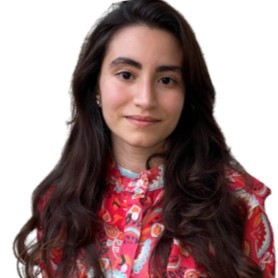
\includegraphics[scale=0.37]{iness.jpeg}
\caption{BOUABID Iness}
\end{minipage}

\begin{minipage}{0.25\textwidth}\
\centering
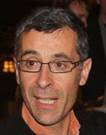
\includegraphics[scale=1.15]{pierre.jpg}
\caption{MARET Pierre}
\end{minipage}
\label{fig:team-presentation}
\end{center}


\subsection{Disponibilités}
\begin{center}
\begin{tabular}{|p{5cm}|p{5cm}|}
\hline
\rowcolor[HTML]{FFFFFF}
\textbf{\color{black}{\makecell{Membre}}} & \textbf{\color{black}{\makecell{Disponibilités}}} \\
\hline
\rowcolor[HTML]{EFEFEF}
BENGUEZZOU Idriss & Mercredi soir, Jeudi soir, Vendredi soir \\
\hline
\rowcolor[HTML]{EFEFEF}
MEZIANE Ghilas & Mercredi soir, Jeudi soir, Vendredi soir \\
\hline
\rowcolor[HTML]{EFEFEF}
BOUABID Iness & Vendredi soir, Samedi soir, Dimanche soir \\
\hline
\rowcolor[HTML]{EFEFEF}
BOUGASSAA Ali & Lundi soir, Mercredi soir, Jeudi soir \\
\hline
\end{tabular}
\end{center}


\subsection{Répartition des tâches et des responsabilités}
Notre projet se décompose en 6 lots livrables: \\
\begin{itemize}
    \item Lot 1 : Définition de l’application.
    \item Lot 2 : Sources de données (au moins 3 sources dans 3 formats) : descriptions, fonctions d’extraction d’informations.
    \item Lot 3 : Interaction avec l’utilisateur.
    \item Lot 4 : Création, alimentation, interrogation de la Wikibase.
    \item Lot 5 : Intégration, test.
    \item Lot 6 : Suivi du projet, communication.


\begin{minipage}{0.25\textwidth}\

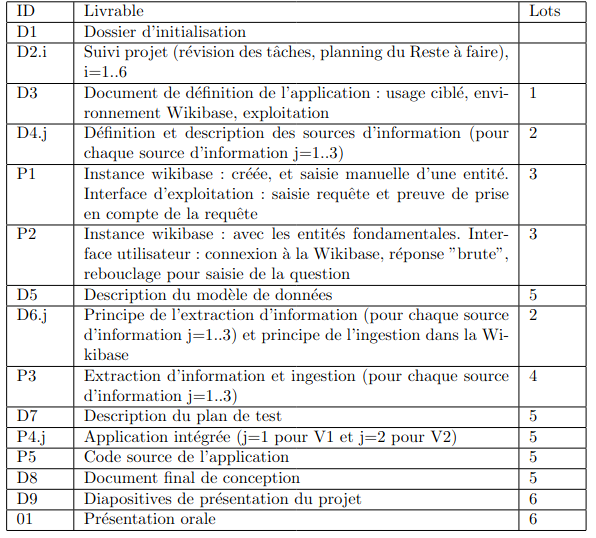
\includegraphics[scale=0.6]{livrables.png}

\end{minipage}

\end{itemize}
\\
Ci dessous la répartition des tâches par membre : \\
\begin{itemize}
    \item MEZIANE Ghilas sera en charge des livrables D1, D2, D4.j P4.j, P2, P5, D7, D9, 01
    \item BENGUEZZOU Idriss sera en charge des livrables D1, D2, D4.j, P4.j, P2, P5, D5, D9, 01
    \item BOUGASSAA Ali sera en charge des livrables D2, D3, D4.j, P2, P4.j, D8, D9, 01
    \item BOUABID Iness sera en charge des livrables D1, D2, D4.j, P1 ,P2, D5, D9, 01
\end{itemize}


    

\end{document}